\documentclass[apectratio=169]{beamer}
\usetheme{metropolis}           % Use metropolis theme
% For PDFs
\newcommand{\myast}{\ensuremath{^{\ast}}}
\newcommand{\mydagger}{\ensuremath{^{\dagger}}}
\usepackage{pdfpages}
\usepackage{minted}
\usepackage{siunitx}
\title{Enabling Ambient Backscatter\\
Using a Low-Cost Software Defined Radio}
\subtitle{Saving Energy/Low Power Communications}
\date{\vspace{1em}
\today}
\author{Maximilian Stiefel\myast, Elmar van Rijnswou\myast\\Carlos Pérez-Penichet\myast, Ambuj Varshney\myast, Christian Rohner\myast and Thiemo Voigt \mydagger
\\\myast Uppsala University
\\\mydagger Uppsala University and RISE SICS
}
\institute{13th Swedish National Computer Networking Workshop}
\begin{document}
  \maketitle

\begin{frame}{Table Of Contents}
  \setbeamertemplate{section in toc}[sections numbered]
  \tableofcontents[hideallsubsections]
\end{frame}

\section{Introduction}
\begin{frame}{What is Backscattering? (1)}
	\begin{figure}[H]	
		\centering
		\only<1>{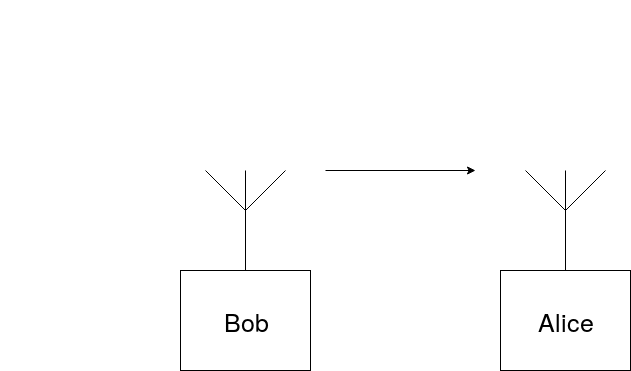
\includegraphics[width=0.8\textwidth]{./fig/backscatter1}}
		\only<2>{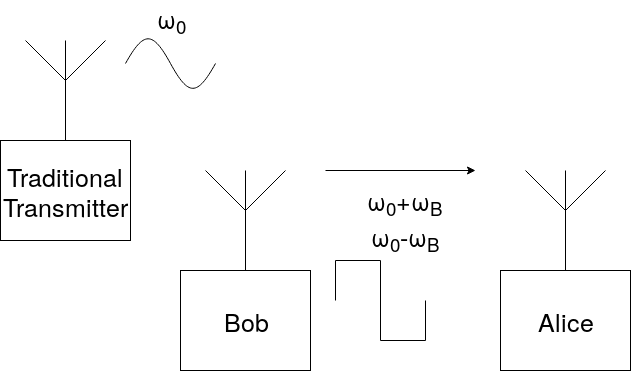
\includegraphics[width=0.8\textwidth]{./fig/backscatter2}}
		\caption{Simplest form of backscattering.}
	\end{figure}
\end{frame}

\begin{frame}{What is Backscattering? (2)}
	\only<1->{\begin{figure}[H]	
		\centering
		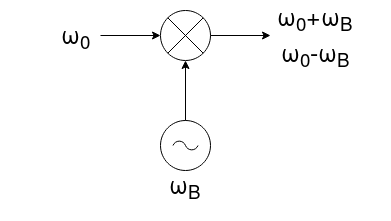
\includegraphics[width=0.6\textwidth]{./fig/mixer}
		\caption{Classical communications engineering element: The mixer.}
	\end{figure}}
	\only<2->{\begin{equation}
	2\sin(f_c t) \sin(\Delta f t) = \cos[(f_c + \Delta f)t] - \cos[(f_c - \Delta f) t]
	\label{eq:mixing}
	\end{equation}}

\end{frame}

\begin{frame}{What is Backscattering? (3)}
	\only<1->{\begin{figure}[H]	
		\centering
		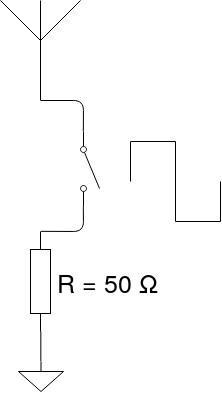
\includegraphics[height=0.5\textheight]{./fig/rfswitch}
		\caption{\SI{50}{\ohm} connected to a RF switch do the trick.}
	\end{figure}}
	\only<2->{
		\begin{equation}
			\Gamma = \frac{Z_L - Z_A}{Z_L + Z_A}
		\end{equation}
	}
\end{frame}

\begin{frame}{Why Backscattering?}
	\begin{itemize}
		\item<1-> Ultra-low power wireless transmissions by reflecting/absorbing EM waves (in orders of \SI{}{\micro\watt}) \cite{liu_ambient_2013}
		\item<2-> Leverage existing signals such as coming from WiFi \cite{hitchhike,kellogg2015wi} or TV towers \cite{liu_ambient_2013,parks_turbocharging_2014}
		\item<3-> Mechanism of choice to network devices operating on harvested energy
		\item<4-> Communication frontends are much simpler, smaller and cheaper, than traditional RF frontends
	\end{itemize}
\end{frame}

\begin{frame}{Contributions}
	\begin{itemize}
		\item<1-> We designed the first system using the RTL-SDR to receive ambient-backscatter.
		\item<2-> We demonstrate ambient backscatter using TV signals to be feasible in wider parts of the city, which is a significant improvement since the state-of-the-art is restricted to a TV towers proximity. 
	\end{itemize}
\end{frame}

\section{Background}
\begin{frame}{RTL-SDR Hardware and I/Q Demodulation (1)}
	\begin{figure}[H]	
		\centering
		\only<1>{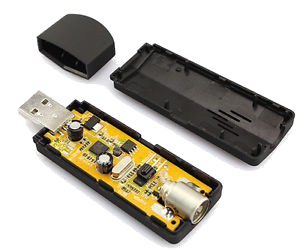
\includegraphics[width=0.7\textwidth]{./fig/rtlsdr}}
		\only<2>{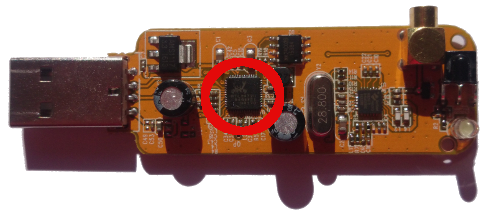
\includegraphics[width=0.7\textwidth]{./fig/rtlsdr1}}
		\only<3>{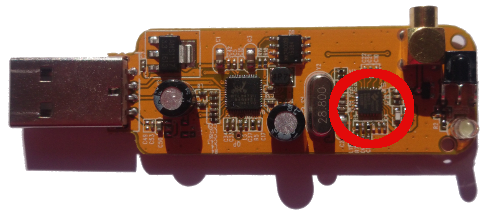
\includegraphics[width=0.7\textwidth]{./fig/rtlsdr2}}
		\caption{RTL-SDR hardware with the DVB-T I/Q demodulator
		Raeltek RTL2832U (left IC) and the tuner with integrated LNA
		Rafael Micro R820T/2 (right IC).}
	\end{figure}
\end{frame}

\begin{frame}{RTL-SDR Hardware and I/Q Demodulation (2)}
	\only<1->{Impinging signal: 
	\begin{equation}
		s_{\text{RF}}(t)=I(t) \cdot cos(\omega_{0}t) + Q(t) \cdot sin(\omega_{0}t)
	\end{equation}}
	\only<2->{Mixing with local RF frequency:
	\begin{multline}
		s_{\text{RF}}(t) \cdot s_{\text{LO}}(t) = I(t) \cdot cos(\omega_{0}t) \cdot cos(\omega_{0}t)\\+ Q(t) \cdot sin(\omega_{0}t) \cdot cos(\omega_{0}t)
	\end{multline}}
	\only<3->{With \ensuremath{2\,cos(a)cos(b)=cos(a-b)+cos(a+b)} and \ensuremath{2\,sin(a)cos(b)=sin(a+b)+sin(a-b)} follows
	\begin{multline}
		        2 \cdot s_{\text{RF}}(t) \cdot s_{\text{LO}}(t) = I(t) \cdot \bigl[1+cos(2\omega_{0}t)\bigr]\\+ Q(t) \cdot \bigl[sin(2\omega_0t)+sin(0)\bigr].
	\end{multline}}

\end{frame}

\section{Design}
\begin{frame}{Transmitter}
	\only<1->{\begin{figure}[H]	
		\centering
		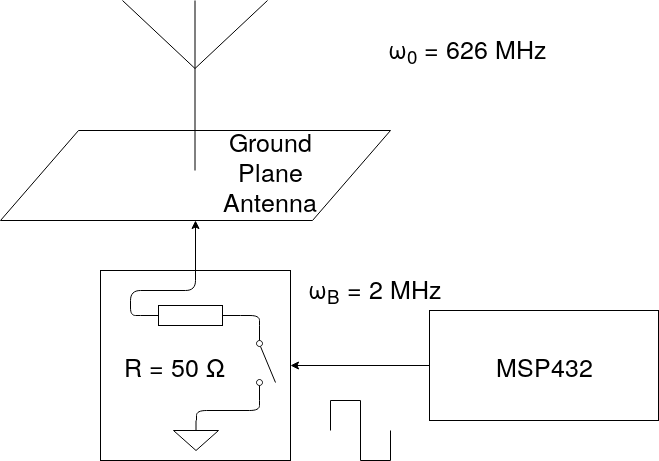
\includegraphics[width=0.7\textwidth]{./fig/transmitter}
		\caption{Transmitter architecture. The ground plane antenna is roughly tuned to the center frequency of the TV signal, which is \SI{626}{\mega\Hz}. A microcontroller steers a RF switch with a rectangular signal to shift the TV wave in another band.}
	\end{figure}}
\end{frame}

\begin{frame}{Receiver (1)}
	\begin{figure}[H]	
		\centering
		\only<1>{
\includegraphics[width=0.9\textwidth]{./fig/receiver1}}
		\only<2>{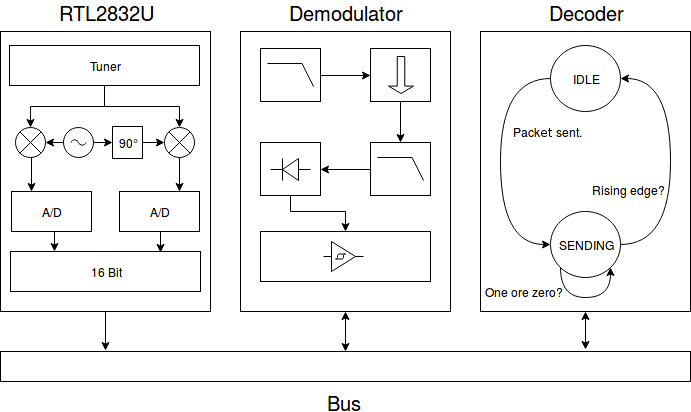
\includegraphics[width=0.9\textwidth]{./fig/receiver2}}
		\caption{Design of the ambient backscatter receiver. The flow
		of operation of the receiver is from the left to right. Code is publicly available under \cite{s3xm3x_backscatterBASKReceiver}.}
	\end{figure}
\end{frame}

\begin{frame}{Receiver (2)}
	\only<1->{The received signal can be interpreted as:
	\begin{equation}
		        I+j\,Q = abs(I,Q) \cdot e^{j \cdot ang(I,Q)} 
	\end{equation}}
	\only<2->{
	Rectification:
	\begin{equation}
		abs(I,Q) = \sqrt{I^2 +  Q^2}
	\end{equation}}
\end{frame}

\section{Evaluation}
\begin{frame}{Spatial Variation of Ambient TV Signals (1)}
\begin{figure}[h]
	\centering
	\begin{minipage}{0.49\columnwidth}
		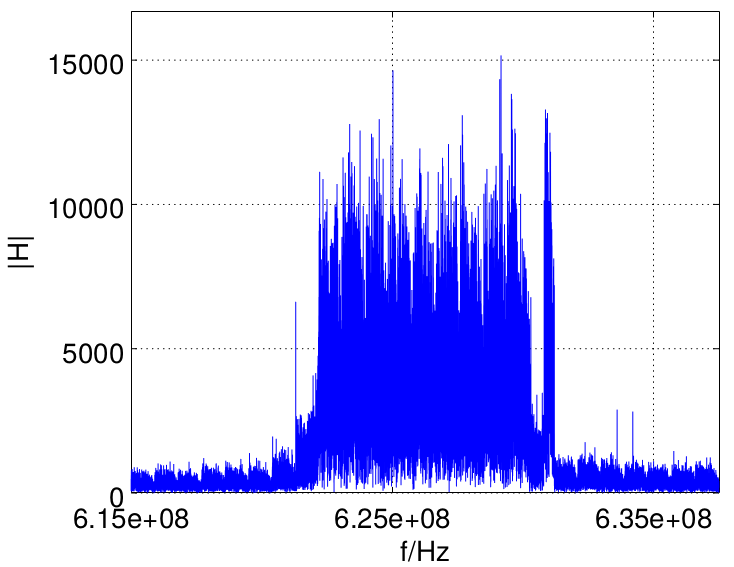
\includegraphics[width=\columnwidth]{./fig/626mhz_raw}
	\end{minipage}
	\hfill
	\begin{minipage}{0.49\columnwidth}
		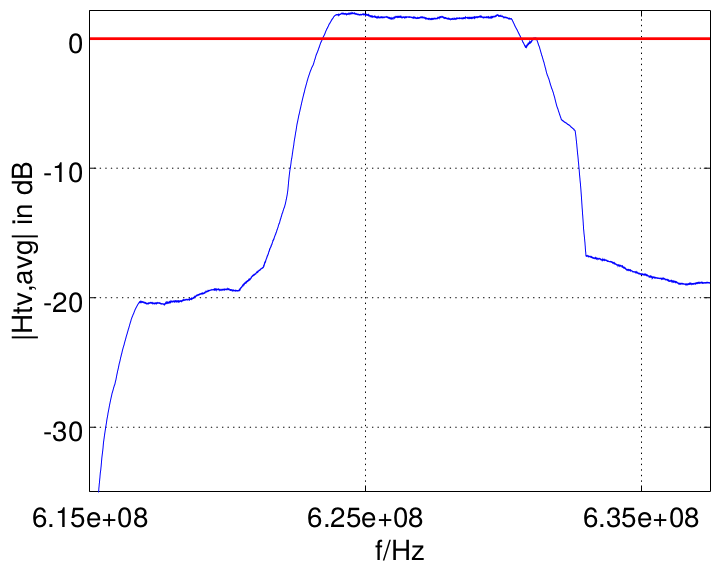
\includegraphics[width=\columnwidth]{./fig/626mhz_filtered}
	\end{minipage}
	\caption{\emph{Observed spectrum of television signal}. The left hand image shows the raw spectrum of the TV signal, with centre frequency of \SI{626}{\mega\hertz}. The right hand image shows the smoothed spectrum normalized to maximum average. The average is  shown by the horizontal red line.}
	\label{fig:tv_record} 
	\end{figure}
\end{frame}

\begin{frame}{Spatial Variation of Ambient TV Signals (2)}
	Perform FFT and stick bands together.
	\begin{equation}
		|H| = \Biggl| \sum_{n=0}^N FFT\biggl( \Re\{ s_{\text{band,n}}(t) \} \biggr) \Biggr|
	\end{equation}
	Smoothing and signal strength calculation. 
	\begin{equation}
		|H_{\text{tv,avg}}| = 20 \cdot log (|H|) - 20 \cdot log(|H_0|)
	\end{equation}
	This has been done with Octave \cite{s3xm3x_RTLSDRSpecAn}.
\end{frame}

\begin{frame}{Spatial Variation of Ambient TV Signals (3)}
\begin{figure}[h]
	\centering
	\begin{minipage}{0.49\columnwidth}
		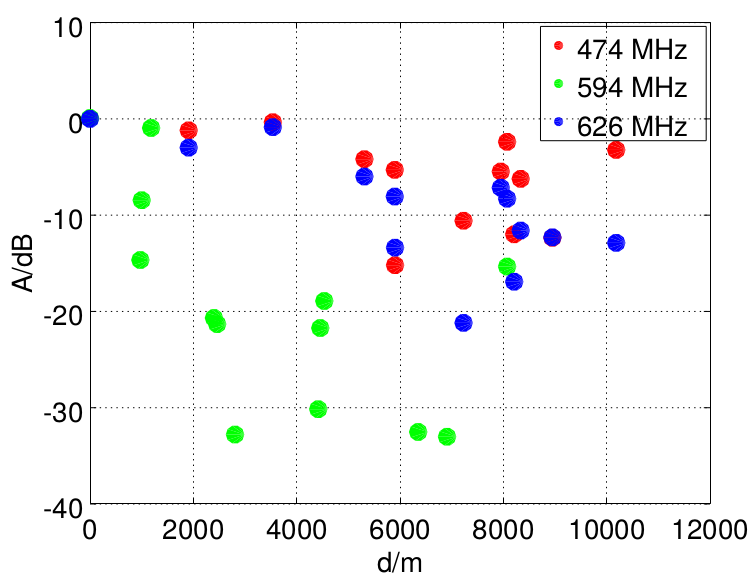
\includegraphics[width=\columnwidth]{./fig/haversine}
	\end{minipage}
	\hfill
	\begin{minipage}{0.49\columnwidth}
		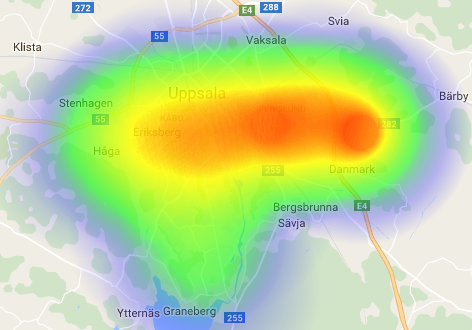
\includegraphics[width=\columnwidth]{./fig/heatmap_626mhz}
	\end{minipage}
	\caption{\emph{Spatial variation of TV signals in Uppsala city}. The left image demonstrates the signal strength of TV signal fading as opposed to observed signal strength near the TV tower. The right image visualises the signal strength as heatmap for the signal present in the \SI{626}{\mega\hertz} band. Distances have been calculated with the Haversine formula. }
	\label{fig:haversine}
\end{figure}
\end{frame}

\begin{frame}{Communication Performance (1)}
	\begin{figure}[h]
	\centering
	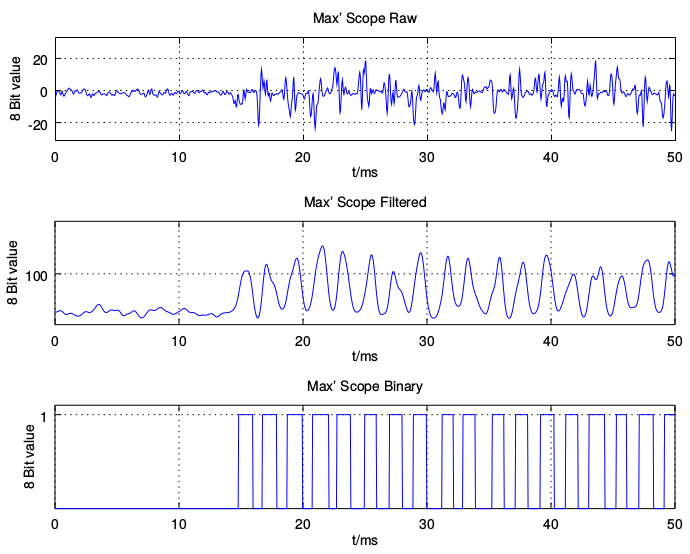
\includegraphics[width=0.5\textwidth]{./fig/transmission}
	\caption{\emph{Plots from Octave oscilloscope showing the start of a transmission of 101010..} In the top plot one can see the raw analog signal, in the middle plot the filtered signal and finally at the bottom the signal after processing though the Schmitt trigger. The amplitude is quite low with an average of 12 \% of the maximum, which is 127.5 due to a low signal strength. Sampling frequency is 25 kHz. }
	\label{fig:transmission}	
\end{figure}
\end{frame}

\begin{frame}{Communication Performance (2)}
	\begin{itemize}
		\item<1-> We varied the bitrate between 1 bit/s and 1 kbit/s 
		\item<2-> Strength of the backscattered signal is quite low (high quantisation noise)
		\item<3-> Higher bitrates (1 kbit/s) lead to a range of a couple of decimeter before the bitrate goes up rapidly (40 \%)
		\item<4-> We acknowledge the high bit errors observed due to primarily limited gain available on the low cost dongles
	\end{itemize}
\end{frame}

\section{Discussion}

\begin{frame}{Discussion}
	\begin{itemize}
		\item<1-> Our system has a lot of space for improvement
		\item<2-> Other antennas for reception and transmission have to be tried out
		\item<3-> The standard cable and the antenna of the RTL-SDR (included in the 10 USD budget) are unsuiteable for our application as we realized
		\item<4-> The filters involved are setscrews as well as the coding used by the communication system (currently none)
	\end{itemize}
\end{frame}

\begin{frame}{Results}
	\begin{itemize}
		\item<1-> We showed thath spectrum scanning over a huge band is possible using the RTL-SDR.
		\item<2-> We found by carrying out a TV signal strength survey that the city is adequate for backscatter communication using our receiver.
		\item<3-> We have shown for the first time, that backscatter communication is possible with the RTL-SDR.
	\end{itemize}
\end{frame}

\begin{frame}{Contact Information}
        	\begin{center}
                \begin{table}[]
                        \begin{tabular}{ll}
                                E: & Elmar.Vanrijnswou.9818@student.uu.se \\
                             	E: & Maximilian.Stiefel.8233@student.uu.se\\
            				& \\
			
\includegraphics[width=0.05\textwidth]{./fig/github} & \url{https://github.com/elamre}\\ 
	& \url{https://github.com/m3x1m0m}
		
		\end{tabular}
                \end{table}

        	\end{center}
        	\begin{figure}
                	
\includegraphics[width=0.3\textwidth]{./fig/logo}
        	\end{figure}
  	\end{frame}

\begin{frame}[standout]
	Happy Coding :) 
\end{frame}

\begin{frame}[allowframebreaks]{References}

  \bibliography{presentation}
  \bibliographystyle{ieeetr}

\end{frame}

\end{document}
